%%%%%%%%%%%%%%%%%%%%%%%%%%%%%%%%%%%%%%%%%%%%%%%%%%%%%%%%%
%                 File: UV1310cdc.tex               	%
%                  Date: 10 Oct, 2015                	%
%                                                    	%
%   For submission to a OFC      						%
%                                                     	%
%   Technical paper about the results obtained with   	%
%   professor Wei Shi with tunable cascaded				%
%	contra-directional coupler				      		%
%	+ theorical analysis								%
%%%%%%%%%%%%%%%%%%%%%%%%%%%%%%%%%%%%%%%%%%%%%%%%%%%%%%%%%



\documentclass[letterpaper,10pt]{article}
\usepackage{osameet2}

\usepackage[utf8]{inputenc} %encoding of the input(this text file)
\usepackage[T1]{fontenc} 	%uses the right font encoding
\usepackage{lmodern,textcomp}		%makes font work for fontenc

\usepackage{ulem}
\usepackage{amsmath,amssymb}

\usepackage{graphicx,epsfig,epstopdf}

\usepackage{xcolor}
\newcommand\todo[1]{\textcolor{red}{#1}}
\renewcommand\todo[1]{}  %activate to get rid of comments

\begin{document}

\title{O-Band Silicon Photonic Bragg-Grating Multiplexers Using UV Lithography}

\author{Jonathan St-Yves, Sophie Larochelle, and Wei Shi$^*$}
\address{Centre d'optique, photonique et laser (COPL) and Département de génie électrique, Université Laval, 2375 rue de la Terrasse, Québec (Québec), Canada, G1V 0A6}
%\email{jonathan.st-yves.1@ulaval.ca}
\email{$^*$wei.shi@gel.ulaval.ca}

\begin{abstract}
We demonstrate the first Bragg-grating-based 4-channel O-band (de-)multiplexer fabricated using 193nm lithography on submicron-SOI with small features below 140nm.
\end{abstract}

\ocis{ (130.7408) Wavelength filtering devices; (350.2770) Gratings; (130.3120)   Integrated optics devices}

\maketitle

\todo{A careful proof reading!!!  The spelling checker was not on in my Overleaf, so there might be quite errors.  Ask for help, e.g., Diane, if needed.}


\section{Introduction}

Integrated optical filters are key components for next-generation optical communications systems enabling cloud services, video streaming, and other data-heavy applications. Applying wavelength division multiplexing (WDM) in data centers allows fibers to transport more information, which requires high-performance, low-cost filters and multiplexers that work in the O-band near 1310 nm, where the chromatic dispersion in conventional fibers is minimal.
Integrated WDM on the submicron silicon-on-insulator (SOI) platform can be achieved using lattice filters\cite{horst2013cascaded} or arrayed waveguides \cite{okamoto2013fabrication}, which, nevertheless, have relatively large footprints and limited free-spectral ranges (FSRs). Others  approaches include Bragg gratings\cite{simard2012apodized} and micro-ring filters\cite{xu2006cascaded}. However, conventional Bragg gratings work in the reflection mode, requiring circulators or interferometers for add-drop operation. Micro-rings suffer from small FSRs and narrow bandwidths. In addition, most existing SOI filters are in C-band, while O-band may be more important for short-reach applications.

Contra-directional couplers (contra-DCs) are Bragg-grating assisted add-drop filters that offer large bandwidth, flat-top response, compact footprint, and high sidelobes suppression \cite{shi2013siliconContraDC}. High-performance coarse WDM using contra-DCs has been demonstrated at 1550 nm using e-beam lithography \cite{shi2013siliconCWDM}. It is critical to implement these devices using deep-ultraviolet lithography for mass production, which is challenging since they 
require small features for gratings \cite{shi2013coupler}. This issue is more significant for 1310 nm applications as the shorter wavelength requires smaller features such as grating pitch and coupler gap.

In this paper, we propose a novel contra-DC geometry in a rib waveguide to increase the mode coupling and thus relax the requirement for small features. The design is implemented using a CMOS-compatible process with 193 nm lithography and a phase-shift mask.  We present the first results of a 4-channel Bragg (de-)multiplexer in O-band with high sidelobe suppression.

\section{Device design and performance}
\subsection{Design} 
\begin{figure}[htbp]
	\centering
	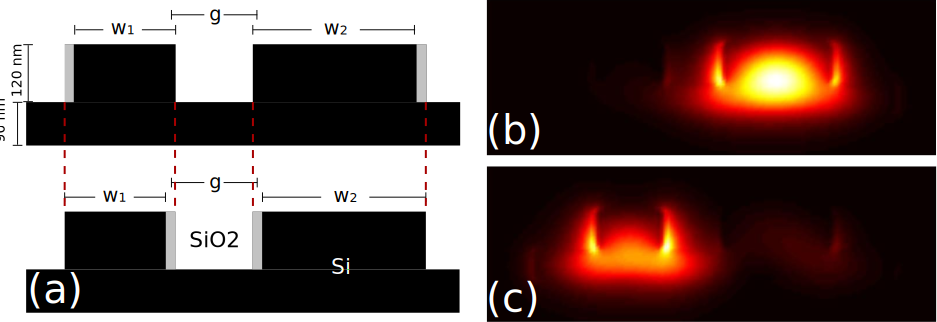
\includegraphics[width=.65\columnwidth]{CrossSection3}
	\caption{ a)Schematics of the cross-section over a period when close (top) and far (bottom): $w_1$ and $w_2$ are the waveguide widths, and $g$ the average gap. b) and c) Intensity distribution of the first and second supermodes. }
    \vspace{-20pt}
	\label{fig:Device}
\end{figure}

The contra-DC filters and cascaded multiplexers are designed for the standard 220-nm SOI wafer. Each contra-DC consists of two waveguides in proximity, with a periodic dielectric perturbations, i.e., Bragg gratings, in the gap region. This introduces wavelength-selective, contra-directional coupling at  $\lambda_\text{c} = \Lambda (n_\text{1}+n_\text{2})$, where $\Lambda$ is the grating pitch, and $n_\text{1}$ and $n_\text{2}$ are the effective indices of the first-order and second-order eigenmodes in the coupler. 
The waveguide coupler is highly asymmetric to suppress the co-directional coupling that would occur with two identical waveguides.

Figure \ref{fig:Device} shows the schematic cross-section of the proposed structure and simulated mode profiles. We observe that the mode confinement is relatively weak due to the small waveguide widths (220 nm and 360 nm) and the existence of the slab in between. Therefore, there is a much stronger mode overlap with the corrugations, compared to the previously demonstrated device in strip waveguide. This allows for stronger coupling, which enables a large bandwidth with a relatively large feature size. The contra-DCs are apodized to reduce side-lobes using a gaussian profile in the coupling with an apodization index $a=10$, following the method described in \cite{shi2013siliconContraDC}.They have 1000 corrugations, measure 400  \textmu m long and 5  \textmu m wide.

\subsection{Fabrication}
The fabrication was performed using a CMOS compatible silicon photonic process with deep UV (193 nm) lithography at IME, Singapore. A phase shift mask is applied, which allows high precision for small features such as grating corrugations. 
Figure \ref{fig:litho} b) shows the SEM image of a device on a separate wafer without oxide cladding. We can see clearly see the grating corrugations, even though the square shaped corrugations in the layout design are smoothed in the lithography as expected. Corrugations with a small period of 260 nm and gaps under 140 nm are resolved.
However, the width of the waveguide along the coupling apodization profile is uneven due to the approximation effect in optical lithography. This results in effective index variations along the propagation direction and thus distortion of the apodization profile, as seen in the measured spectra to be discussed below.

\begin{figure}[htbp]
	\centering
	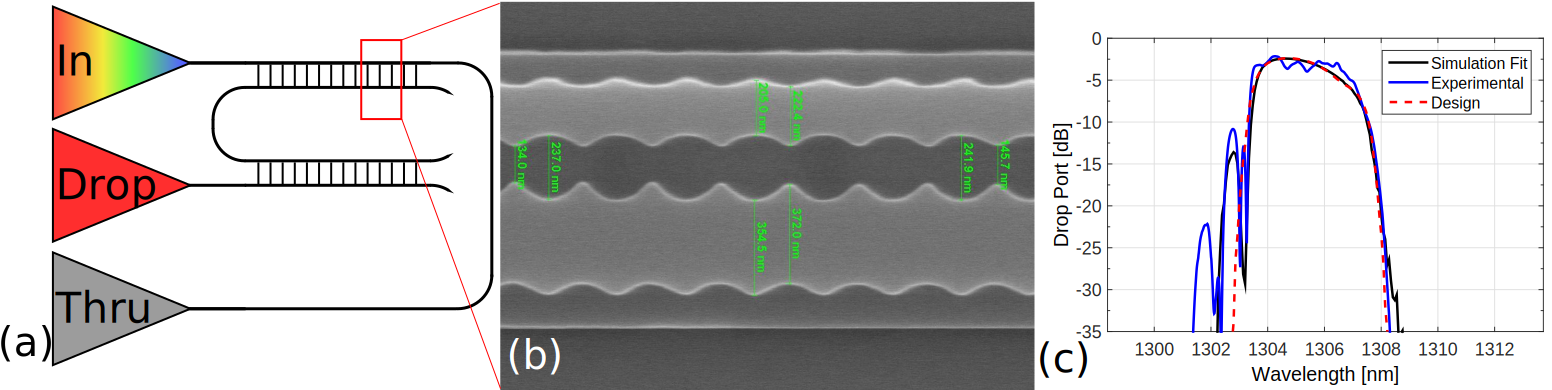
\includegraphics[width=.99\columnwidth]{SingleFilterFig}
	\caption{ a) Schematic of a dual-stage single-channel contra-DC. b)SEM showing that the waveguide widths vary in the close and far regions. c) Simulated and measured spectral response of the dual-stage contra-DC, with fiber-to-chip response subtracted.}
	\vspace{-20pt}
    \label{fig:litho}
\end{figure}

\subsection{Experimental results}
Figure \ref{fig:litho} c) shows the spectral response of a dual stage filter. The insertion loss is 2.5 dB with a 1-dB bandwidth covers 370 GHz. A sidelobe suppression ratio of 8 dB is obtained, which is lower than the results (> 20 dB) achieved with the devices fabricated using e-beam lithography \cite{shi2013siliconCWDM}. This is explained by the variations in corrugations and effective indices due to fabrication errors. 
As a result, the effective indices in the strong coupling regions are higher than in the weak coupling regions, which creates undesired a coupling dependent chirp, i.e., phase noise along the grating apodization profile. Taking this coupling dependent chirp into consideration, our simulation fits well with experimental results. With this information, we will be able to bias future devices to compensate for the optical lithography impact and significantly improve the performance.

%\subsection{WDM performance}
\begin{figure}[htbp]
	\centering
	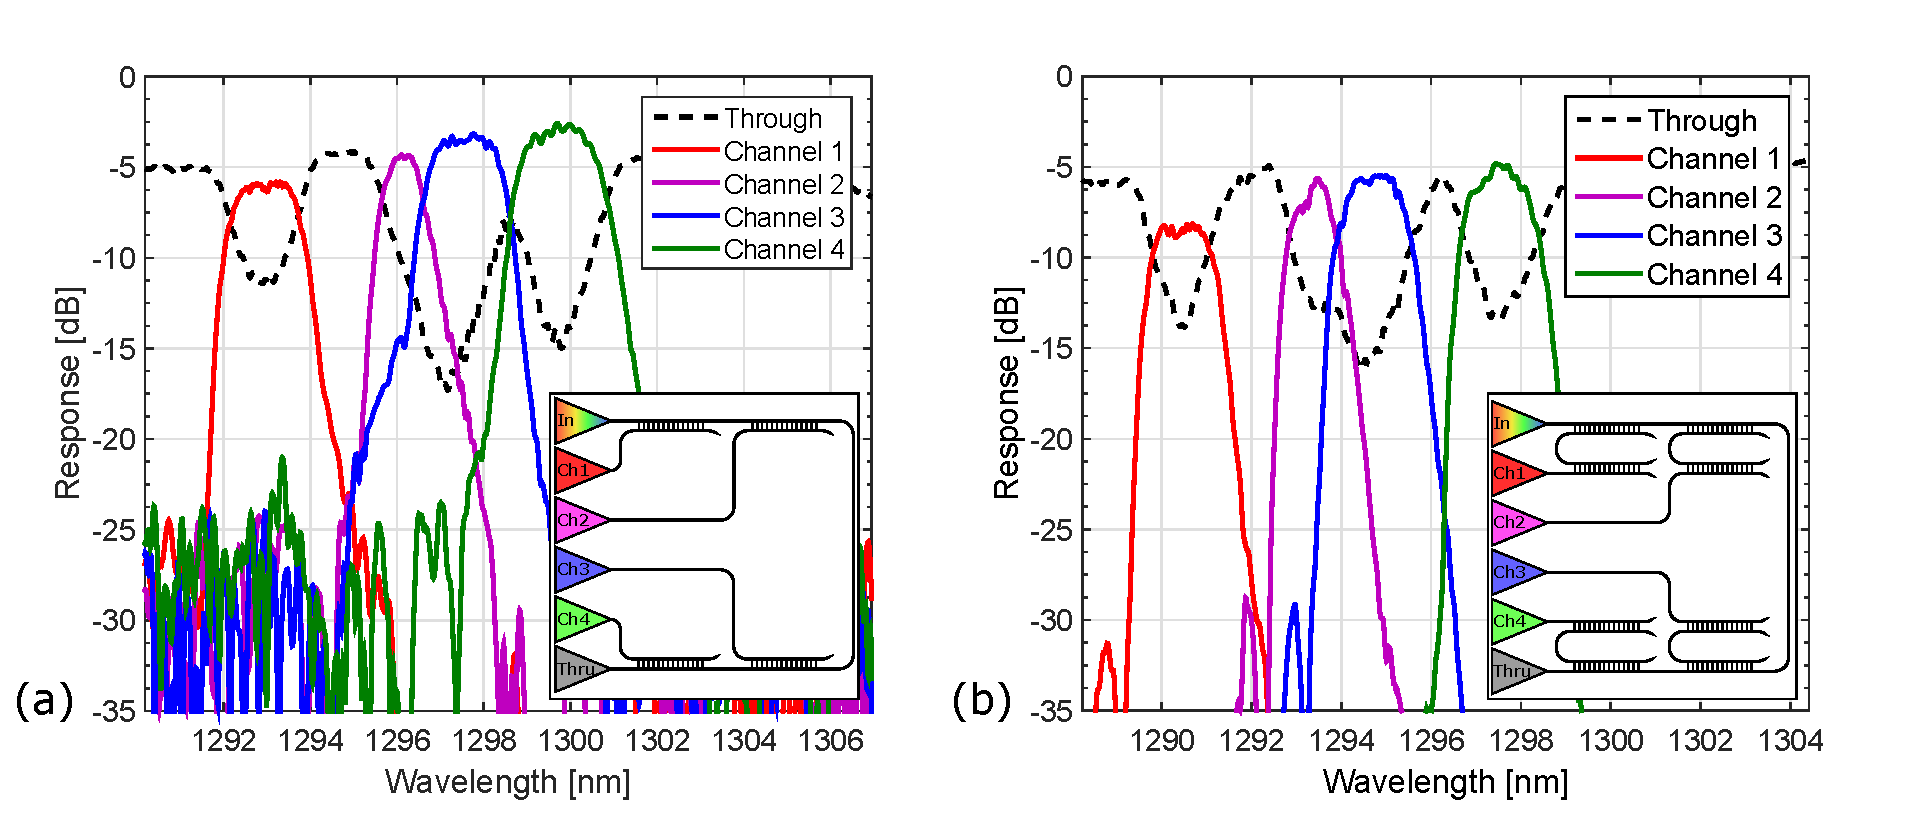
\includegraphics[width=.8\columnwidth]{WDM}
	\caption{Measured spectra of contra-DC demultiplexers: a) single-stage; b) dual-stage.}
    \vspace{-15pt}
	\label{fig:WDM}
\end{figure}

Figure \ref{fig:WDM} shows the performance of two 4-channel wavelength demultiplexers. The device (Fig.~\ref{fig:WDM}a) consists of four contra-DCs cascaded along a bus waveguide. 
The second one (Fig.~\ref{fig:WDM}b) applies dual-stage filtering for a lower crosstalk. The contra-DCs in different channels have slightly different pitch ($\Lambda$) for specific wavelengths. The channels are dropped in a reverse order such that a shorter wavelengths go through more contra-DCs and thus a longer waveguide path. This explains why the loss increases as the channel wavelength decreases. An obvious problem is that the second channel has a smaller bandwidth than the others and its center wavelength is off the design grid. 
We believe this is due to the quantization errors in the grating pitch definition in the mask layout and should be avoided in the future using precise control of the center wavelength by varying the waveguide widths. As shown in Fig.~\ref{fig:WDM}b, other channels without suffering from this error have shown good performance with a low crosstalk below -25 dB. 
%This is a systematic glitch in all the devices we measured, caused by the fact that channel 2 has an even grating pitch of 260 nm and that the grid resolution of the fabrication is 1 nm, causing it to snap differently to the grid than the other devices. This causes its effective index and central wavelength to be slightly higher.

\section{Conclusion}
In summary, we demonstrated, for the first time, Bragg-grating-based multiplexers in the O-band on submicron SOI using UV lithography. This technology is a key enabler for low cost and flexible WDM in data centers. 
The prototype presented gives the community critical information about the possible issues when using UV lithography for small features and how to consider them for future designs.

\section*{Acknowledgments}
We acknowledge CMC Microsystems for the access to the design software and fabrication process. The authors acknowledge the Natural Sciences and Engineering Research Council (NSERC) of Canada for funding this research. This work is part of the SPEED research project funded by NSERC, PROMPT, and TeraXion.

\bibliographystyle{osajnl}
\bibliography{bibli}

\end{document}